\chapter{Introduction to Photogrammetry}

If recapping - skip to the "Better Explanation" section.

This chapter was taught using Computational Photogrammetry by Cyrill Stachniss.

Computer Vision came into being because cameras existed that could image things. Let's consider a pinhole camera - it assumes that all rays will come through the pinhole and it can use these rays to project an image onto another screen. The image is hence, a projection of points in a 3D world to a 2D surface. Camera center is the intersection point of the rays. The back wall is the image plane. The distance between the camera center and image plane is the camera constant.

We'll assume that all our cameras for the next sections are pinhole cameras. 

\textbf{Geometry and Images}

Pinhole cameras have some properites: The straight lines are preserved, lengths are not preserved, and angles between lines change. Additionally, parallel lines may intersect depending on the angle at which the image is taken.

Image rectification is a transformation process used to project images onto a common image plane. Photogrammetry deals with such problems - the relationship between the object in the scene and the object in the image, the image and the rays in the object, the orientation of cameras in the scene, and infer geometry of an object or a scene given an object.

Photogrammetry is hard because information is lost when a scene is projected onto a surface by a camera. There is a loss of depth and 3D information cannot be recovered from this information alone - additional information required. 

\textbf{Vanishing Points}

Parallel lines aren't always parallel if taken at an angle and they intersect at a vanishing point - at infinity. This information cannot classically be represented using cartesian coordinates $(x, y)$. Euclidian geometry is suboptimal to describe the central projection. Projective geomtry is an alternate representation of geometric objects and transformations. With projective geometry, the math becomes simpler

Hence, we need a new representation for coordinates which is homogeneous coordinates.

\section{Homogeneous Coordinates}

Homogenous coordinates are for projective geomtry just as cartesian coordinates are for Euclidian geometry. Formulas involving H.C. are often simpler than in the Cartesian world. The points at infinity can be represented using finite coordinates. Further, complex projective transformations can be represented using a single matrix! 

"The  ideas and notation of projective geometry are central to an analysis of multiple view geometry.For example, the use of homogeneous coordinates enables non-linear mappings (such as perspective projection) to be represented by linear matrix equations, and points at infinity  to  be  represented  quite  naturally  avoiding  the  awkward  necessity  of  taking limits." from \href{https://github.com/pranjals16/cs676/blob/master/Hartley\%2C\%20Zisserman\%20-\%20Multiple\%20View\%20Geometry\%20in\%20Computer\%20Vision.pdf}{this}.

\textbf{Notation}

\begin{itemize} 
    \item Point $\chi$: In homogenous it is x, in euclidian $x$
    \item Line in homogeneous coordinates is l.
    \item Plane in homogenous coordinates : A
\end{itemize}

The representation x of a geometric object is homogenous if x and $\lambda$x represent the same object for $\lambda \neq 0$. H.C uses a n+1 dimensional vector to represent the same point:

\begin{equation}
    x = \begin{bmatrix}
    x \\
    y
    \end{bmatrix} \text{ and x = } \begin{bmatrix}
    x \\
    y\\
    1
    \end{bmatrix}
\end{equation}

Note that in general for a point $x = (x, y)^T$ and a line $l: ax + by + c = 0$ satisfies $x \cdot l = 0$. 

\begin{figure}[t]
    \centering
    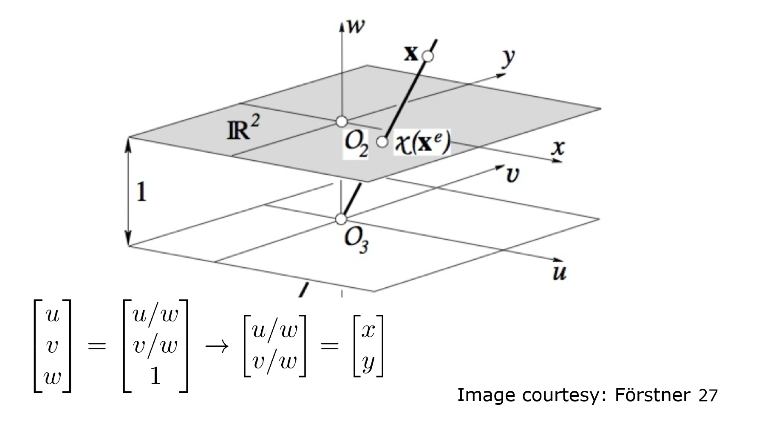
\includegraphics[width=10cm]{img/homogenous-eucclidian.png}
    \caption{Homogeneous Coordinates Representation/Visualization}
    \label{fig:hc}
\end{figure}

Before coming to the image notation, it is useful to look at section 2.2.1 of \href{https://github.com/pranjals16/cs676/blob/master/Hartley\%2C\%20Zisserman\%20-\%20Multiple\%20View\%20Geometry\%20in\%20Computer\%20Vision.pdf}{Multiple View Geometry in Computer Vision by Hartley, Zisserman}. The book is a great source of information. I would've written that explanation myself but it's hard to do it better than that.

Summary: A point in a 2D plane can be represented as a 3D column vector, and when multiplied by a constant k, it still represents the same point - just on the line that may be scaled by the same constant. It is natural, therefore, to consider the set of vectors $(kx, ky, k)^T$ for varying values of $k$ to be a representation of the point $(x, y)^T$ in $R^2$. Thus, just as with lines, points are represented by homogeneous vectors. An arbitrary homogeneous vector representative of a point is of the form $x=(x_1,x_2,x_3)^T$, representing the point $(x1/x3,x2/x3)^T$ in $R^2$. 

Refer to figure \ref{fig:hc}.

Let us assume that we have a 2D plane that is our image. Now, different points on this image can be visualized to have certain rays passing through it. If we look at the diagram, the point x is a point on the ray that can be represented with our scaling factor/H.C. value. The origin $O_3$ is where the rays originate from (camera center). In fact, we cannot have this origin point in our coordinate system since if the image has this point, then there is no direction for any of the rays. Hence homogenous coordinates of a point $\chi$ in the plane $R^2$ is a 3-dim vector.

\begin{equation}
    \chi: \; x = \begin{bmatrix}
    u/w \\
    v/w 
    \end{bmatrix}
     \text{ with $w\neq 0$ }
\end{equation}

Now, if $w$ is 0, then that is essentially our understanding of a point at infinity in the direction of $u$ and $v$ (notice how $u/0$ is infinity!). The projective plane (the grey plane) contains all points $\chi$ of the Euclidian plane $R^2$ with $x = [x, y]^T$ expressed through a 3 valued vector and all points at infinity (x = $[x, y, 0]^T$ except $[0, 0, 0]^T$).

Additionally, it can be seen that our homogeneous property is like the depth of the point/distance from camera center.

\subsection{Representation of Lines}

Refer to slides 31+ \href{https://github.com/RoboticsIIITH/summer-sessions-2020/blob/master/lecture-slides/Computational\%20Photogrammetry/Projective\%20Geometry\%20Lecture\%201.pdf}{here}.

There is a duality between lines and points when we talk about them (they are both 3D vectors!!). 

\subsection{The Better Explanation}

I did not understand any of this until I read \href{https://pointatinfinityblog.wordpress.com/2016/04/11/points-at-infinity-i-projective-geometry/}{this resource} by points at infinity. It is very well-written but a gist could be:

\begin{enumerate}
    \item We can look at projective planes (which we represent with homogeneous coordinates) as a window through which we see the 3D world. Previously, we used the idea of a pinhole camera. Rather than that, imagine that you are looking at a real building or so. Now, if we had to paint this/capture this image, we will trace a line from a point on the building to our eye. This is a line in 3D euclidian space. This line becomes a point in projective $P^2$ space!
    \item Note that if we know a point on a line, if we multiply it with a scalar, we get a new point on the line! ($x + y + z = 0 \implies \alpha(x+y+z)=0)$. Hence, the entire set of points in 3D space that lie on the same line from the building to our eye can be represented by a single line which in turn is a point in projective plane!
    \item Now if a line in 3D is a point in projective plane, a plane in 3D is a line in projective plane. Imagine this this way: when we trace a line on our image of a building, we can imagine that we are drawing a line on the window through which we see the building. Further, this line can slowly be moved back (like the points on the line that connected our eye and the building). Now, we see that the line on our image, when extended became a plane! The representation for the line is also with a 3D vector. 
    \item We have already seen that for a line (a 3D euclidian line) represented by $(a, b, c)$, the point in projective plane can be represented with $(a, b, c)$ as well but for ease, we tend to use $(a/c, b/c, 1)$. Further, if we capture the image, the coordinate for this point can be imagined as $(a/c, b/c)$.  
    \item Points at 3D: The main reason to move towards projective plane is to introduce the idea of parallel lines convering at infinity. When we have a line with $c=0$, this means that our image point is $\infty, \infty)$ or rather, the line ends at infinity! This is precisely why parallel lines intersect at infinity in a projective plane! 
\end{enumerate}

\subsection{Intersecting Lines}

If we have two lines $l, m$ that intersect at a point $x$, then x will satisfy both line equations or:

\begin{equation*}
\begin{bmatrix}
l\cdot x \\
m\cdot x
\end{bmatrix} = \begin{bmatrix}
0 \\
0
\end{bmatrix}
\end{equation*}

\subsubsection{Cramer's Rule}

Given a system of linear equations, Cramer's Rule is a handy way to solve for just one of the variables without having to solve the whole system of equations. If we have a system of equations, let $D$ be the coefficient matrix's determinant. $D_X$ is the determinant of coefficient matrix which has the solution vecctor in the $x-\text{column}$. As per cramer's rule, $x = D_x / D $. Now, for this $2 \times 2$ system, we will find that $D_1 = l_2m_3 - l_3m_2$ and $D_2 = l_3m_1 - l_1m_3$ and $D_3 = l_1m_2 - l_2m_1$. Looking at this closer will tell us that the coordinate/point x is actually $l \times m$ (the cross product)!.

Similarly, we can show that the line that passes through two points is represented by the cross product of these two points. 

\subsection{Parallel Lines and ideal points}

Read section 2.2.2 of the multi view book to look at how parallel lines intersect at infinity! There is honestly nothing better to understand. I'm also very dead atm.2